\begin{appendices}
    \chapter{Detailed Results of Questionnaire}
    \label{sec:detailed_questionnaire_results}

    \begin{figure}[H]
        \centering
        \resizebox{0.85\textwidth}{!}{
        \begin{tabular}{| c | c | c | c | c |}
            \hline
            \textbf{problem} & \textbf{impact} & \textbf{difficulty} & \textbf{likelihood} \\ \hline
            charging\_failure & [1, 2, 1, 1, 2, 1, 1] & [1, 2, 1, 2, 1, 1, 1] & [2, 2, 2, 1, 3, 1, 1] \\ \hline
            incorrect\_localization & [2, 1, 1, 2, 1, 2, 2] & [2, 3, 2, 2, 3, 2, 2] & [2, 2, 2, 1, 1, 2, 1] \\ \hline
            power\_management & [1, 1, 1, 1, 1, 1, 1] & [1, 1, 1, 3, 1, 2, 1] & [2, 3, 2, 1, 2, 2, 2] \\ \hline
            data\_management & [1, 2, 2, 2, 2, 1, 1] & [2, 2, 3, 1, 2, 2, 2] & [1, 2, 2, 2, 2, 2, 2] \\ \hline
            sustained\_recovery & [1, 2, 1, 2, 1, 1] & [2, 2, 2, 3, 3, 3] & [2, 2, 1, 2, 3, 2] \\ \hline
            mapping\_error & [2, 2, 1, 2, 2, 2, 2] & [2, 3, 1, 2, 3, 2, 2] & [2, 2, 2, 1, 1, 2, 2] \\ \hline
            navigation\_failure & [1, 1, 3, 2, 2, 2, 2] & [2, 1, 2, 3, 2, 2] & [2, 3, 1, 1, 2, 2] \\ \hline
            robot\_gets\_stuck & [1, 1, 2, 1, 3, 1, 1] & [2, 3, 3, 1, 3, 2, 2] & [3, 2, 3, 2, 1, 2, 2] \\ \hline
            sensor\_failure & [1, 1, 2, 1, 2, 2, 2] & [1, 1, 2, 2, 2, 2, 2] & [1, 3, 2, 3, 2, 2, 2] \\ \hline
            lost\_connection & [2, 1, 2, 3, 3, 2, 2] & [1, 1, 3, 1, 2, 2, 3] & [2, 1, 3, 1, 1, 1, 2] \\ \hline
            plan\_deployment\_failure & [1, 2, 1, 2, 2, 2] & [2, 1, 2, 2, 2, 2] & [2, 3, 1, 2, 3, 2] \\ \hline
            obstacles\_blocking\_path & [2, 3, 2, 2, 2, 2, 3] & [2, 3, 3, 1, 2, 2, 2] & [2, 1, 3, 1, 1, 1, 1] \\ \hline
            drastic\_weather\_change & [2, 2, 1, 2, 2, 2, 2] & [2, 3, 2, 3, 3, 2, 2] & [3, 2, 2, 2, 3, 2, 2] \\ \hline
            certain\_dynamics & [2, 3, 3, 2, 2, 2, 3] & [2, 1, 1, 3, 1, 1, 1] & [2, 3, 1, 1, 3, 1, 1] \\ \hline
            robot\_falls\_over & [1, 1, 1, 1, 1, 1, 1] & [3, 2, 1, 2, 3, 3] & [3, 3, 2, 3, 2, 3] \\ \hline
            perceptual\_aliasing\_issue & [2, 2, 1, 2, 3, 2] & [2, 2, 3, 3, 3, 2] & [2, 2, 3, 2, 3, 2] \\ \hline
        \end{tabular}}
    \caption{\textsc{Results of the Questionnaire (cf. Section \ref{sec:relevance_assessment})}}
    \label{fig:detailed_res}
    \end{figure}

    \chapter{Detailed Results of Experiments}
    \label{sec:detailed_experiments_results}

    \begin{figure}[H]
        \centering
        \resizebox{\textwidth}{!}{
        \begin{tabular}{| c | c | c | c | c | c | c | c | c | c | c | c | c |}
            \hline
            \textbf{exp.} & \textbf{duration (h)} & \textbf{comp.} & \textbf{tasks} & \textbf{charge cycles} & \textbf{missions} & \textbf{dist. (m)} & \textbf{traverse (s)} & \textbf{scan (s)} & \textbf{wait (s)} & \textbf{charge (s)} & \textbf{dock (s)} & \textbf{undock (s)} \\ \hline
            0 & $5.09$ & True & $100$ & $9$ & $3$ & $1036.39$ & $13751.42$ & $1075.85$ & $0.10$ & $501.25$ & $1330.16$ & $1461.30$ \\ \hline
            1 & $5.04$ & True & $110$ & $10$ & $4$ & $1131.86$ & $12121.07$ & $1060.32$ & $0.17$ & $514.19$ & $1966.06$ & $1770.60$ \\ \hline
            2 & $5.14$ & True & $110$ & $10$ & $4$ & $1139.80$ & $12118.70$ & $1038.16$ & $0.14$ & $493.30$ & $1840.95$ & $1940.00$ \\ \hline
        \end{tabular}}
    \caption{\textsc{Results of the Basic Functionality Experiments}}
    \label{fig:detailed_functionality_res}
    \end{figure}
    \begin{figure}[H]
        \centering
        \resizebox{\textwidth}{!}{
        \begin{tabular}{| c | c | c | c | c | c | c | c | c | c | c | c |}
            \hline
            \textbf{exp.} & \textbf{sim. probs.} & \textbf{correct cont.} & \textbf{correct no-cont.} & \textbf{false pos.} & \textbf{false neg.} & \textbf{unexp. cont.} & \textbf{comp.} & \textbf{tasks} & \textbf{charge cycles} & \textbf{missions} & \textbf{dist. (m)} \\ \hline
            250\_42\_0 & $13$ & $12$ & $1$ & $0$ & $0$ & $0$ & True & $88$ & $11$ & $3$ & $904.09$ \\ \hline
            250\_42\_1 & $15$ & $12$ & $2$ & $0$ & $1$ & $1$ & True & $72$ & $9$ & $2$ & $872.58$ \\ \hline
            250\_42\_2 & $12$ & $11$ & $1$ & $1$ & $0$ & $0$ & True & $93$ & $12$ & $3$ & $1014.08$ \\ \hline
            250\_42\_3 & $13$ & $12$ & $1$ & $0$ & $0$ & $0$ & True & $90$ & $10$ & $3$ & $991.41$ \\ \hline
            250\_42\_4 & $15$ & $12$ & $2$ & $0$ & $1$ & $0$ & True & $99$ & $10$ & $4$ & $1043.19$ \\ \hline
            250\_42\_5 & $8$ & $7$ & $1$ & $0$ & $0$ & $0$ & False & $45$ & $5$ & $2$ & $543.86$ \\ \hline
            250\_42\_6 & $14$ & $12$ & $2$ & $0$ & $0$ & $0$ & True & $82$ & $10$ & $3$ & $944.71$ \\ \hline
            250\_42\_7 & $5$ & $4$ & $1$ & $0$ & $0$ & $0$ & False & $34$ & $5$ & $2$ & $393.04$ \\ \hline
            250\_42\_8 & $12$ & $10$ & $1$ & $0$ & $1$ & $0$ & True & $83$ & $11$ & $3$ & $908.25$ \\ \hline
            250\_42\_9 & $16$ & $14$ & $2$ & $0$ & $0$ & $1$ & True & $103$ & $10$ & $3$ & $1058.45$ \\ \hline
        \end{tabular}}
    \caption{\textsc{Results of the Evaluation of the Monitoring Framework}}
    \label{fig:detailed_monitoring_eval_res}
    \end{figure}
    \begin{figure}[H]
        \centering
        \resizebox{0.7\textwidth}{!}{
        \begin{tabular}{| c | c | c | c | c | c | c | c | c |}
            \hline
            \textbf{exp.} & \textbf{duration (h)} & \textbf{traverse (s)} & \textbf{scan (s)} & \textbf{wait (s)} & \textbf{cont. (s)} & \textbf{charge (s)} & \textbf{dock (s)} & \textbf{undock (s)}  \\ \hline
            250\_42\_0 & $5.06$ & $11625.58$ & $1189.62$ & $53.68$ & $832.23$ & $691.38$ & $2205.18$ & $1561.86$ \\ \hline
            250\_42\_1 & $5.02$ & $11990.75$ & $970.09$ & $26.80$ & $749.50$ & $664.05$ & $2447.46$ & $1007.05$ \\ \hline
            250\_42\_2 & $5.03$ & $11934.69$ & $996.74$ & $24.68$ & $544.81$ & $677.71$ & $1840.19$ & $2008.67$ \\ \hline
            250\_42\_3 & $5.05$ & $12429.86$ & $1069.81$ & $73.06$ & $420.69$ & $603.87$ & $1605.38$ & $1898.25$ \\ \hline
            250\_42\_4 & $5.14$ & $12279.08$ & $1266.11$ & $25.64$ & $487.82$ & $645.02$ & $2120.26$ & $1364.29$ \\ \hline
            250\_42\_5 & $3.11$ & $6232.27$ & $624.24$ & $75.38$ & $368.37$ & $274.08$ & $2236.34$ & $896.04$ \\ \hline
            250\_42\_6 & $5.03$ & $11914.37$ & $1085.09$ & $68.67$ & $394.88$ & $650.74$ & $2080.91$ & $1713.65$ \\ \hline
            250\_42\_7 & $2.30$ & $4909.87$ & $419.87$ & $0.44$ & $271.59$ & $226.10$ & $983.53$ & $985.87$ \\ \hline
            250\_42\_8 & $5.07$ & $11495.68$ & $1024.95$ & $51.77$ & $466.79$ & $679.69$ & $2122.77$ & $2243.42$ \\ \hline
            250\_42\_9 & $5.04$ & $11875.13$ & $1308.44$ & $50.93$ & $801.70$ & $603.96$ & $1490.83$ & $1685.22$ \\ \hline
        \end{tabular}}
    \caption{\textsc{Mode Times in the Evaluation of the Monitoring Framework}}
    \label{fig:detailed_monitoring_eval_mode_times}
    \end{figure}

    \chapter{Considered Mission Plan}
    \label{sec:complete_plan_sec}

    \begin{figure}[H]
        \centering
        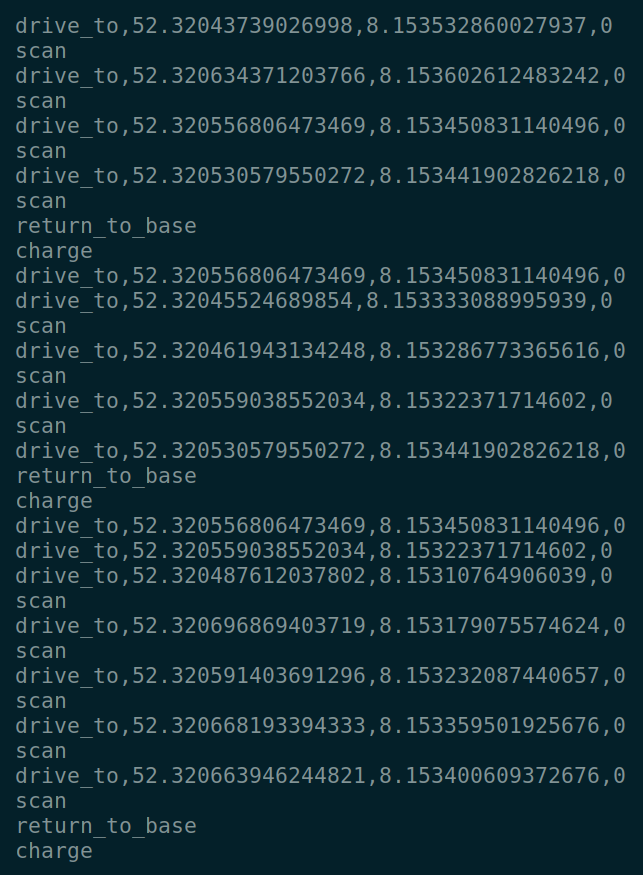
\includegraphics[width=0.5\textwidth]{img/complete_plan.png}
        \caption{\textsc{Complete Plan - Corresponds to the Example Route (cf. fig.\ref{fig:example_scan_route})}}
        \label{fig:complete_plan}
    \end{figure}

\end{appendices}
